\subsection{Ablation Studies}

\subsubsection{Results on platform1}

\begin{table}[t]
\centering
\caption{Ablation results for platform1.}
\label{tab:ablation_platform1}
\scriptsize
\setlength{\tabcolsep}{3pt}
\begin{tabular}{lccc}
\toprule
Variant & RMSE$\downarrow$ & $\Delta$RMSE & Params \\
\midrule
Full Model & 0.34017 & -- & 313.7K \\
\addlinespace[1pt]
w/o Patch & 0.24778 & -27.2\% & 311.4K \\
w/o Attention & 0.34537 & +1.5\% & 48.0K \\
w/o Positional Enc. & \textbf{0.19311}$^\dagger$ & -43.2\% & 313.7K \\
\addlinespace[1pt]
Patch L=2 & 0.32684 & -3.9\% & 312.2K \\
Patch L=4 & 0.44131 & +29.7\% & 313.7K \\
Patch L=8 & 0.25525 & -25.0\% & 316.8K \\
Patch L=16 & 0.45547 & +33.9\% & 322.9K \\
\addlinespace[1pt]
P=4 & 1.33270 & +291.8\% & 313.7K \\
P=8 & 0.27941 & -17.9\% & 313.7K \\
P=16 & 0.27875 & -18.1\% & 313.7K \\
P=32 & 0.25368 & -25.4\% & 313.7K \\
P=64 & 0.22850 & -32.8\% & 313.7K \\
\addlinespace[1pt]
L=1 & 0.64040 & +88.3\% & 114.6K \\
L=2 & 0.41294 & +21.4\% & 214.1K \\
L=3 & 0.25527 & -25.0\% & 313.7K \\
L=4 & 0.24332 & -28.5\% & 413.3K \\
L=6 & 0.22859 & -32.8\% & 612.5K \\
\addlinespace[1pt]
d=12 & 0.27630 & -18.8\% & 302.9K \\
d=32 & 0.21205 & -37.7\% & 306.4K \\
d=64 & 0.23359 & -31.3\% & 313.7K \\
d=128 & 1.49179 & +338.5\% & 334.5K \\
\bottomrule
\end{tabular}
\vspace{2pt}
\raggedright\footnotesize $^\dagger$ Best non-baseline configuration.
\end{table}


\begin{figure}[t]
    \centering
    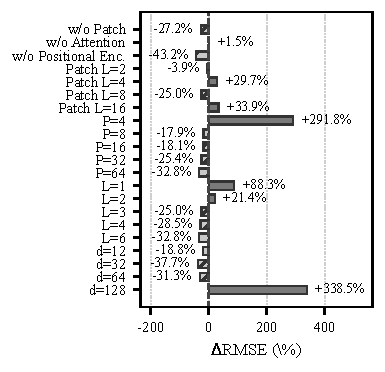
\includegraphics[width=\columnwidth]{fig_ablation_platform1.pdf}
    \caption{Relative RMSE changes of ablation variants on platform1 (flexible manipulator). Attention removal and excessive latent lifting cause the most severe degradation, while positional encoding has only a marginal effect.}
    \label{fig:ablation_platform1}
\end{figure}

Table~\ref{tab:ablation_platform1} and Fig.~\ref{fig:ablation_platform1} show that platform1 mainly benefits from attention-based temporal interaction modeling. Removing attention produces the largest module-level degradation, increasing the rollout RMSE from 0.19248 to 0.51161 (+165.8\%), while removing patching also causes a substantial degradation of +62.6\%. By contrast, removing positional encoding only changes the RMSE by +3.0\%, which suggests that this platform is comparatively insensitive to absolute temporal order once local temporal aggregation is retained.

The hyperparameter ablations further indicate that the default configuration is already close to a strong operating point on platform1. Reducing the Transformer depth to one or two layers clearly harms performance, whereas increasing the depth to four layers yields only a marginal improvement to \textbf{0.18968}$^\dagger$. This small gain suggests that the baseline depth of three layers already captures most of the useful temporal interaction structure. Similarly, moderate changes to patch length and latent dimension only produce limited degradation, but over-expanding the latent dimension to $d=128$ severely worsens the RMSE by +229.5\%, indicating over-parameterized lifting and less stable latent dynamics.

The per-dimension errors are also consistent with this interpretation. For platform1, the error is mainly concentrated in dimensions 1, 3, and 5. Removing attention increases the RMSE of dim1 from 0.2895 to 0.8256 and dim3 from 0.2588 to 0.7427, suggesting that attention is essential for capturing coupled temporal interactions across the multivariate state trajectory.

\subsubsection{Results on platform2}

\begin{table}[t]
\centering
\caption{Ablation results for platform2.}
\label{tab:ablation_platform2}
\scriptsize
\setlength{\tabcolsep}{3pt}
\begin{tabular}{lccc}
\toprule
Variant & RMSE$\downarrow$ & $\Delta$RMSE & Params \\
\midrule
Full Model & 0.79420 & -- & 10.1K \\
\addlinespace[1pt]
w/o Patch & 1.54428 & +94.4\% & 10.1K \\
w/o Attention & 1.83102 & +130.5\% & 806 \\
w/o Positional Enc. & 1.40783 & +77.3\% & 10.1K \\
\addlinespace[1pt]
Patch L=1 & 2.60828 & +228.4\% & 10.1K \\
Patch L=4 & \textbf{0.50643}$^\dagger$ & -36.2\% & 10.2K \\
\addlinespace[1pt]
P=2 & 0.64922 & -18.3\% & 10.1K \\
P=4 & 1.83841 & +131.5\% & 10.1K \\
P=6 & 0.93819 & +18.1\% & 10.1K \\
P=8 & 1.86611 & +135.0\% & 10.1K \\
P=12 & 1.01518 & +27.8\% & 10.1K \\
P=16 & 2.49727 & +214.4\% & 10.1K \\
\addlinespace[1pt]
L=1 & 0.65175 & -17.9\% & 3.5K \\
L=2 & 1.20094 & +51.2\% & 6.8K \\
L=3 & 1.02695 & +29.3\% & 10.1K \\
L=4 & 0.77098 & -2.9\% & 13.4K \\
\addlinespace[1pt]
d=4 & 1.93372 & +143.5\% & 10.0K \\
d=8 & 0.88055 & +10.9\% & 10.1K \\
d=16 & 2.15635 & +171.5\% & 10.4K \\
d=32 & 1.50382 & +89.4\% & 11.5K \\
d=64 & 0.52010 & -34.5\% & 15.2K \\
\bottomrule
\end{tabular}
\vspace{2pt}
\raggedright\footnotesize $^\dagger$ Best non-baseline configuration.
\end{table}


\begin{figure}[t]
    \centering
    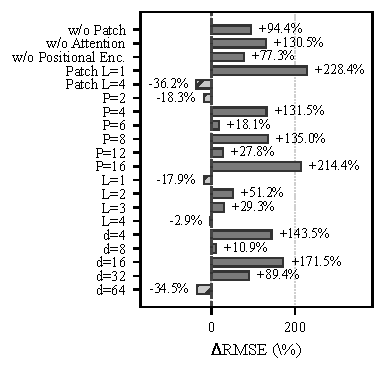
\includegraphics[width=\columnwidth]{fig_ablation_platform2.pdf}
    \caption{Relative RMSE changes of ablation variants on platform2 (soft robot). Unlike platform1, platform2 is highly sensitive to positional encoding and history length, indicating stronger dependence on temporal ordering and longer memory.}
    \label{fig:ablation_platform2}
\end{figure}

platform2 exhibits a different ablation pattern. As shown in Table~\ref{tab:ablation_platform2} and Fig.~\ref{fig:ablation_platform2}, removing positional encoding causes the largest module-level degradation, increasing the RMSE from 0.78149 to 1.82345 (+133.3\%). Removing patching also produces a large degradation (+85.1\%), while removing attention causes a smaller but still substantial increase of +48.5\%. These results indicate that platform2 depends more strongly on temporal ordering information than platform1.

The parameter sweep shows that longer temporal memory is beneficial on platform2. Increasing the history length from the default $P=4$ to $P=8$ reduces the RMSE by 37.1\%, and even the shorter setting $P=2$ still improves over the default baseline by 17.4\%. In addition, reducing the Transformer depth to one layer improves the RMSE by 22.2\%, whereas using two layers causes a dramatic failure case with +279.7\% degradation. A similarly strong deterioration appears when the latent dimension is expanded to $d=32$ (+185.4\%), which indicates that this lower-dimensional system is more vulnerable to over-parameterized temporal lifting.

The per-dimension statistics highlight the source of these failures. Removing positional encoding dramatically increases the RMSE of dim1 from 0.3321 to 2.4798, which suggests that temporal ordering is crucial for platform2. The unstable Layers=2 case mainly comes from dim0, whose RMSE increases from 1.0541 to 4.1818, implying that the deeper temporal encoder can become unstable even when the second state component remains relatively well behaved.

\subsubsection{Cross-Platform Discussion}

The ablation results reveal platform-dependent temporal modeling requirements rather than inconsistency of the proposed framework. On platform1, the dominant factor is attention-based global temporal interaction, while positional encoding has only a marginal effect. On platform2, by contrast, positional encoding and history length are far more important, indicating stronger reliance on temporal ordering and longer effective memory. These results suggest that PatchTST-Koopman adapts to different temporal structures across dynamical systems: platform1 benefits more from global temporal interaction modeling, whereas platform2 depends more strongly on explicit ordering cues and memory length. Therefore, the optimal temporal configuration should be understood as platform-dependent, even though the full PatchTST-Koopman design provides a consistent and effective temporal lifting framework across both systems.
